\documentclass[tikz]{standalone}

\usetikzlibrary{positioning, calc, decorations.pathreplacing}

\begin{document}
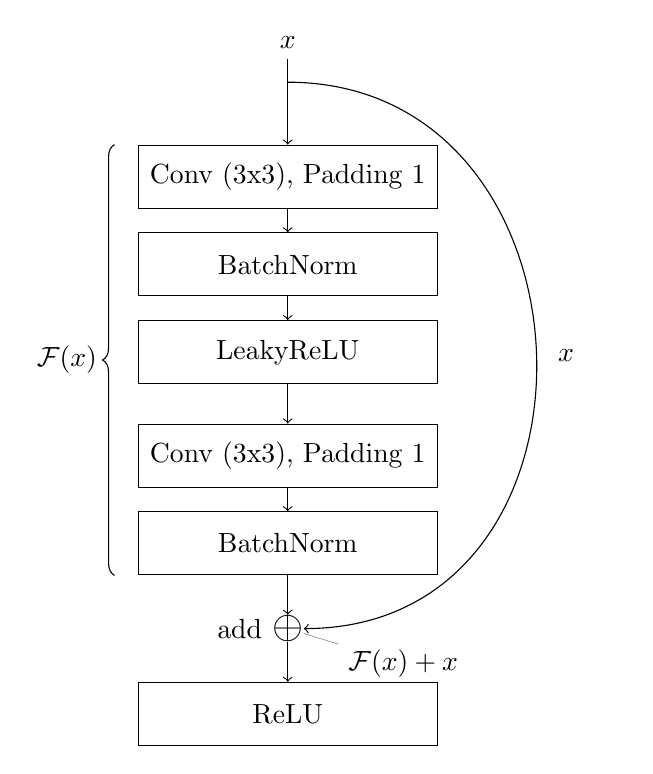
\begin{tikzpicture}

  \node[draw=black, minimum width=3.8cm, minimum height=0.8cm] (conv_1) {Conv (3x3), Padding 1};
  \node[draw=black, minimum width=3.8cm, minimum height=0.8cm, below=0.3cm of conv_1] (bn_1) {BatchNorm};
  \node[draw=black, minimum width=3.8cm, minimum height=0.8cm, below=0.3cm of bn_1] (lr) {LeakyReLU};
  \node[draw=black, minimum width=3.8cm, minimum height=0.8cm, below=0.5cm of lr] (conv_2) {Conv (3x3), Padding 1};
  \node[draw=black, minimum width=3.8cm, minimum height=0.8cm, below=0.3cm of conv_2] (bn_2) {BatchNorm};
  \node[below=0.5cm of bn_2, font=\Large, label={left:add}, inner sep=0, pin={-13:$\mathcal F(x) + x$}] (add) {$\oplus$};
  \node[draw=black, minimum width=3.8cm, minimum height=0.8cm, below=0.5cm of add] (r) {ReLU};

  \draw[<-] (conv_1) -- ++(0,1.5) node[above, pos=1] {$x$};
  \draw[->] (conv_1) -- (bn_1);
  \draw[->] (bn_1) -- (lr);
  \draw[->] (lr) -- (conv_2);
  \draw[->] (conv_2) -- (bn_2);
  \draw[->] (bn_2) -- (add);
  \draw[->] (add) -- (r) node[above, pos=0.8] {};
  \draw[->, looseness=1.5] ($(conv_1)-(0,-1.2)$) to[out=0, in=0] node[right=1ex, midway, align=center] {$x$} (add);
  \draw[decorate, decoration={brace, amplitude=1ex, raise=2.2cm}] (bn_2.south) -- node[midway, left=2.3cm] {$\mathcal F(x)$} (conv_1.north);

\end{tikzpicture}
\end{document}
